\documentclass[a4paper,12pt]{article}
\usepackage{amsmath} \usepackage{amsthm}
\usepackage[croatian]{babel}
\usepackage{graphicx}
\usepackage{amssymb} \usepackage{fancybox}
\usepackage{latexsym}
\usepackage{enumerate}
\usepackage{subfigure}
\addtolength{\hoffset}{-1cm} \addtolength{\textwidth}{2cm}
\addtolength{\topmargin}{-2.5cm} \addtolength{\textheight}{3cm}

\newtheoremstyle{zad}% name
  {0.3cm}%      Space above
  {10pt}%      Space below
  {}%         Body font
  {}%         Indent amount (empty = no indent, \parindent = para indent)
  {\bf}% Thm head font
  {.}%        Punctuation after thm head
  {\newline}%     Space after thm head: " " = normal interword space;
        %       \newline = linebreak
  {}%         Thm head spec (can be left empty, meaning `normal')

\theoremstyle{zad}
\newtheorem{zadatak}{Zadatak}
\DeclareMathOperator{\rand}{\mathrm{rand}}
\DeclareMathOperator{\arctg}{\mathrm{arctg}}
\DeclareMathOperator{\sign}{\mathrm{sign}}

\begin{document}
%\thispagestyle{empty}
\begin{center}
\shadowbox{\Large Svijanje torusa}\\[2pt]
\end{center}
Svijanjem plohe u smjeru njezine normale mogu se dobiti nove plohe s interesantnijim reljefom. Pokazat \'cemo nekoliko
primjera svijanja torusa. Opisane ideje mo\v{z}emo primijeniti na proizvoljnim plohama.\\[5pt] 
Parametarske jednad\v{z}be torusa glase
\begin{align*}
x&=(R+r\cos{v})\cos{u}\\
y&=(R+r\cos{v})\sin{u}\\
z&=r\sin{v}
\end{align*}
pri \v{c}emu su $u,v\in[0,2\pi]$ i $r<R$.

\begin{figure}[!h]
\centering
\subfigure[fiksni manji polumjer]{
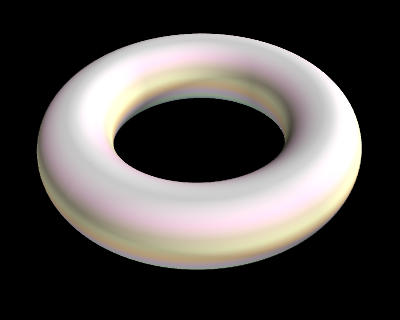
\includegraphics[scale=0.35]{sv_torus1.png}
\label{slika1}}\hspace*{0.5cm}
\subfigure[varijabilni manji polumjer]{
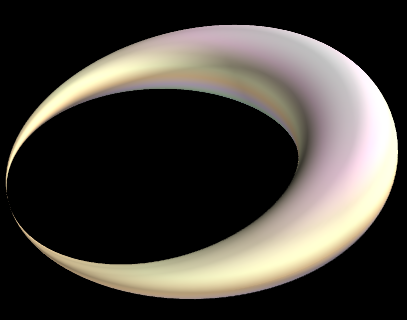
\includegraphics[scale=0.35]{sv_torus2.png}
\label{slika2}}
\vspace*{-10pt}
\caption{Torus}
\label{slika12}
\end{figure} 

\noindent Stavimo li u parametarske jednad\v{z}be torusa varijabilni manji polumjer $r=\sin^2{\frac{u}{2}}$, dobivamo plohu s parametarskim jednad\v{z}bama
\begin{align*}
x&=\big(R+\sin^2{\tfrac{u}{2}}\cos{v}\big)\cos{u}\\[2pt]
y&=\big(R+\sin^2{\tfrac{u}{2}}\cos{v}\big)\sin{u}\,.\\[2pt]
z&=\sin^2{\tfrac{u}{2}}\sin{v}
\end{align*}

\noindent Neka je $\mathbf{x}(u,v)=\big((R+r\cos{v})\cos{u},\,(R+r\cos{v})\sin{u},\,r\sin{v}\big)$ parametrizacija torusa.\vspace*{2pt} Jedini\v{c}na normala u proizvoljnoj to\v{c}ki torusa dobiva se po formuli
$$\mathbf{n}(u,v)=\frac{\mathbf{x}_u\times\mathbf{x}_v}{\|\mathbf{x}_u\times\mathbf{x}_v\|}$$
pri čemu su $\mathbf{x}_u$ i $\mathbf{x}_v$ parcijalne derivacije vektorske funkcije $\mathbf{x}$.\\[5pt]
Ploha prikazana na slici \ref{sl3} dobiva se periodi\v{c}kim svijanjem torusa u smjeru njegove jedini\v{c}ne normale. Njezina parametrizacija glasi
$$\mathbf{y}(u,v)=\mathbf{x}(u,v)+2\cdot|\sin{5u}+\sin{3v}|\cdot\mathbf{n}(u,v).$$

\begin{figure}[!h]
\centering
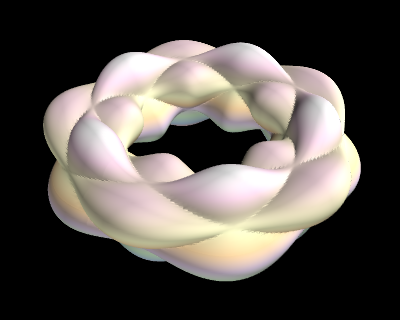
\includegraphics[scale=0.35]{sv_torus3.png}
\vspace*{-5pt}
\caption{Svijanje torusa}\label{sl3}
\end{figure}

\noindent U nastavku dalje navodimo dvije varijante slu\v{c}ajnog svijanja torusa. 
Neka je $\rand(a,b)$ funkcija koja na slu\v{c}ajni na\v{c}in vra\'ca neki realni broj na segmentu $[a,b]$. Za odabrane $m,n\in\mathbb{N}$ def\mbox{}iniramo funkciju
$$f(u,v)=\sum_{i=0}^n\sum_{j=0}^m{\rand(-1,1)\cdot\cos{\big(iu+2\pi\cdot\rand(0,1)\big)}\cdot\cos{\big(jv+2\pi\cdot\rand(0,1)\big)}}.$$
Na kraju za odabrani $h\in\mathbb{R}$ def\mbox{}iniramo plohu parametrizacijom
$$\mathbf{r}_1(u,v)=\mathbf{x}(u,v)+h\cdot f(u,v)\cdot\mathbf{n}(u,v).$$

\begin{figure}[!h]
\centering
\subfigure[$\mathbf{r_1}(u,v)$]{
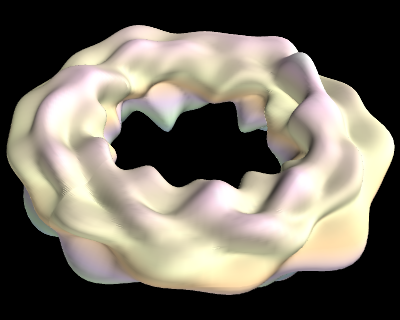
\includegraphics[scale=0.34]{sv_torus4.png}
\label{slika4}}\hspace*{0.5cm}
\subfigure[$\mathbf{r_2}(u,v)$]{
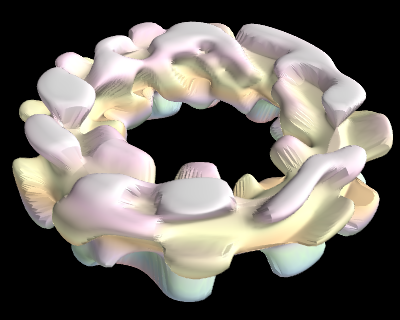
\includegraphics[scale=0.34]{sv_torus5.png}
\label{slika5}}
\vspace*{-10pt}
\caption{Random svijanje torusa}
\label{slika45}
\end{figure}

\noindent Na slici \ref{slika4} prikazana je ploha s parametrizacijom $r_1$ i odabranim parametrima\linebreak $R=10,\,r=3,\,h=0.2,\,n=12,\,m=6$.\\[8pt] 
Za vektore $\mathbf{u}=(u_1,u_2,u_3)$ i $\mathbf{v}=(v_1,v_2,v_3)$ def\mbox{}iniramo operaciju $\ast$ formulom
$$\mathbf{u}\mathrel{\ast}\mathbf{v}=\big(u_1v_1,\,u_2v_2,\,u_3v_3\big).$$
Za vektor $\mathbf{u}=(u_1,u_2,u_3)$ i realnu funkciju realne varijable $g$ def\mbox{}iniramo $g(\mathbf{u})$ formulom
$$g(\mathbf{u})=\big(g(u_1),\,g(u_2),\,g(u_3)\big).$$
Na primjer, 
\begin{itemize}
\item za $g(x)=|x|$ je $|\mathbf{u}|=\big(|u_1|,\,|u_2|,\,|u_3|\big)$
\item za $g(x)=\arctg{x}$ je $\arctg{\mathbf{u}}=\big(\arctg{u_1},\,\arctg{u_2},\,\arctg{u_3}\big)$ 
\item za $g(x)=x^{\frac{2}{3}}$ je $\mathbf{u}^{\frac{2}{3}}=\Big(u_1^{\frac{2}{3}},\,u_2^{\frac{2}{3}},\,u_3^{\frac{2}{3}}\Big)$
\end{itemize}
Za odabrani realni broj $\varepsilon$ i vektor $\mathbf{v}$ def\mbox{}iniramo funkciju skaliranja $s$ formulom
$$s(\mathbf{v})=\sign{\mathbf{v}}\mathrel{\ast}\left(\tfrac{2}{\pi}\arctg{\mathbf{|v|}}\right)^{\varepsilon}.$$
Kona\v{c}no, def\mbox{}iniramo plohu parametrizacijom
$$\mathbf{r}_2(u,v)=\mathbf{x}(u,v)+h\cdot s\big(f(u,v)\cdot\mathbf{n}(u,v)\big).$$

\noindent Na slici \ref{slika5} prikazana je ploha s parametrizacijom $r_2$ i odabranim parametrima\linebreak $R=10,\,r=3,\,h=1,\,n=12,\,m=6,\,\varepsilon=0.5$.\\[8pt]
Konačno, odgovarajućim translacijama možemo sve navedene plohe razmjestiti kako je prikazano na slici \ref{svi_torusi}.

\begin{figure}[!h]
\centering
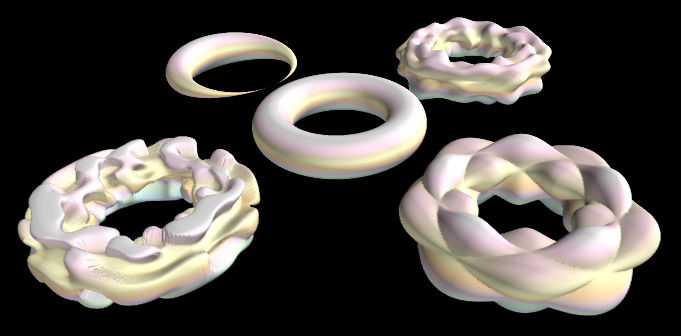
\includegraphics[scale=0.35]{sv_torus6.png}
\vspace*{-5pt}
\caption{3D scena s torusima}
\label{svi_torusi}
\end{figure}

\end{document}
